\subsection{知識}

  \subsubsection{HL7 \cite{bibi5} \cite{bibi6} }
  HL7とはHealth Level Sevenの略称である.
  医療情報システム間のISO-OSI第7層アプリケーション層に由来している.
  2015年11月現在,国内で約20の企業が会員となっている.
  特定の部門やシステムに特化したものでなく,施設間・システム間での
  臨床情報や管理情報を扱い,相互運用性を高めるための
  ヘルスケア領域でのデータ交換標準である.

  データ定義は図\ref{ss-mix_sample}のようになっている.
  また,図\ref{ss-mix_sampledata}が
  その出力データのサンプルである.


	\begin{figure}[htbp]
		\begin{center}
			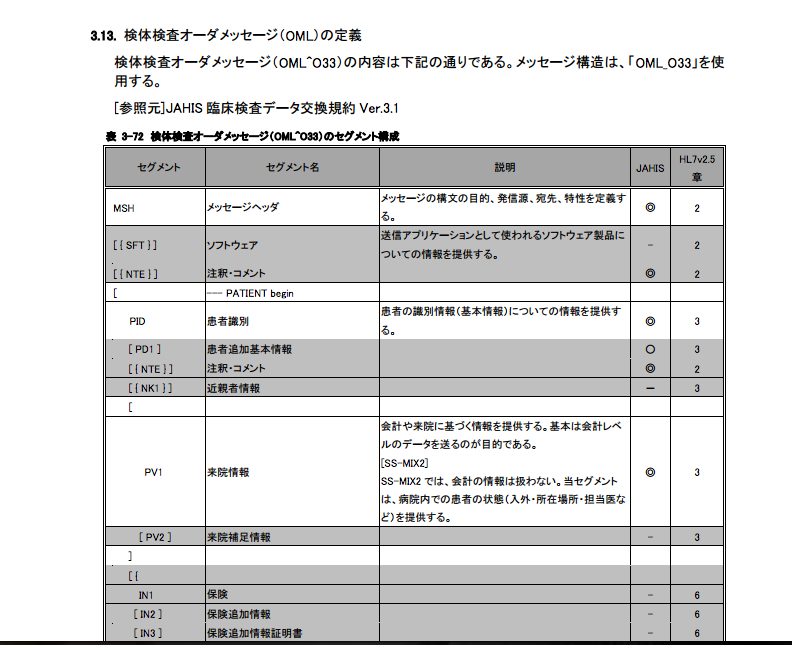
\includegraphics[width=5cm, bb=0 0 645 790]{./gazou/ss-mix_sample.png} %よこたて
		\end{center}
		\caption{データ定義}
		\label{ss-mix_sample}
	\end{figure}

	\begin{figure}[htbp]
		\begin{center}
			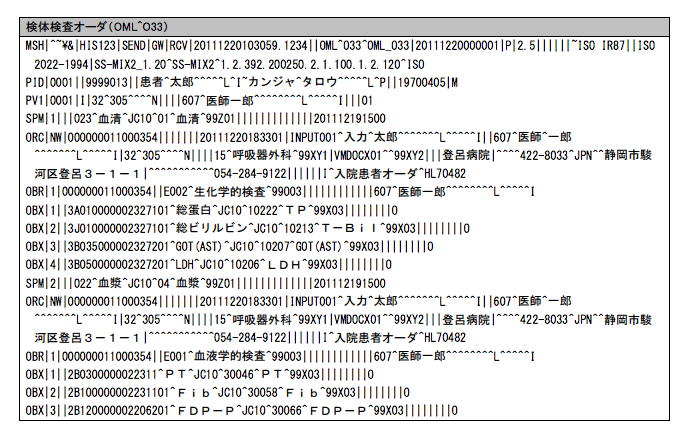
\includegraphics[width=5cm, bb=0 0 437 688]{./gazou/ss-mix_sampledata.png}
		\end{center}
		\caption{データサンプル}
		\label{ss-mix_sampledata}
	\end{figure}



  \subsubsection{SQL,NoSQLについて}



\subsection{本研究の類似製品,研究}
  後述する既存アプリID-Linkなどは患者idをリンクしているだけで
  情報を一元的に集約はしていない.

  \subsubsection{ID-Link}
    ID-Linkは地域内の病院の患者IDを一元管理することで,
    地域内の病院で作られた電子カルテを参照することができるシステムである.
    医療情報そのものは収集していない.データセンターには患者IDのリンクが
    あるだけで,病院間を安全な通信技術で結び,相互参照させている.
    患者には事前に情報共有に関する許可をもらうことが通例になっている.
    シェアは2015年2月末に全国で4300の機関である.

  \subsubsection{SS-MIX} \cite{bibi7}
    SS-MIXは医療情報を収集するために,平成18年から動き出した
    厚生労働省を中心としたプロジェクトである.
    これは標準規格がないまま立ち上がった電子カルテの医療情報の
    電子化についての標準規格である.SS-MIXで規格化された
    基本情報,処方歴,検査結果を各機関のストレージに収集する.
    診断時に医師用端末から参照することや,紹介情報を作るときにも
    情報を引き出すことができる.
    これにはHL7が採用されている.

  \subsubsection{あじさいネット}\cite{bibi3}
    2004年に長崎県大村市で始まり、2012年には,
    県域をカバーする地域医療連携ネットワークとして発展してきた.
    2013年4月現在において,電子カルテなどの患者情報の提供を
    行う地域の機関的病院は17病院,地域の診療所や調剤薬局などの
    情報閲覧施設は178施設,医療関係者の会員数は285名を数え,
    これまでに同意を得て登録された患者数は2万6千人を超えている.

    あじさいネットは10年にわたる活動の中でアンケートを繰り返し,
    会費だけで運用することができるシステムになっていった.
